\chapter{Music Playlist Generation}\label{final}
\section{DATA SET }

\textbf{last.fm-dataset-360K}

March 2010

Version 1.2


\textbf{Dataset has two files} :-
\begin{enumerate}
\end{enumerate}

1. First file(usershal-profile.tsv) contains general information about users

	\textbf{columns} = [user , gender , age, country, signup]

2. Second file(usersha1-artmbid-artname-plays.tsv) contains information about user and artist song plays

		\textbf{columns} = [user, musicbrainz-artist-id, artist-name, plays]



\section{Dataset Preprocessing and modification}

user-profile pre-processing

\textbf{columns} = [user, country]

user-artist-plays file pre-processing

\textbf{columns} = [user, artist-name, plays]

Unpopular artist are removed and after some modification final data set

\textbf{columns} = [user, artist-name, plays, total artist plays, country]



\section{K-Nearest Neighbour\cite{code}}
We have looked at various collaborative approaches like Latent factor model and matrix factorization method. we have used KNN model on last.fm data set to form recommendation system.

Basically, KNN algorithm assumes that similar thing exist in close proximity. we have to define a distance function to find distance between two points (could be as simple as Manhattan distance or Cartesian's distance). Then using this function we find K nearest neighbour to the query point.

\textbf{Pseudo Code}

Initialize K to your chosen number of neighbors

1. For each example in the data

1.1 Calculate the distance between the query example and the current example from the data.

1.2 Add the distance and the index of the example to an ordered collection

2. Sort the ordered collection of distances and indices from smallest to largest (in ascending order) by the distances

3. Pick the first K entries from the sorted collection

4. Get the labels of the selected K entries

5. If regression, return the mean of the K labels

6. If classification, return the mode of the K labels

we have eliminated unpopular artist means only those artist are taken whose total count is greater than \textbf{popularity threshold} which is a hyper parameter. In current implementation we have kept this number to be 1,00,000. We have also taken only \textbf{American user} mainly to reduce data. This is also a hyper parameter.
Then on this reduced data, KNN model is trained.

\section{Playlist Generation}
We will generate top 100 recommendation using our music recommendation model and out of these 100, 10(These 10 will be chosen based on shuffling algorithm discussed in next chapter ) will be used as playlist. 

\begin{figure}
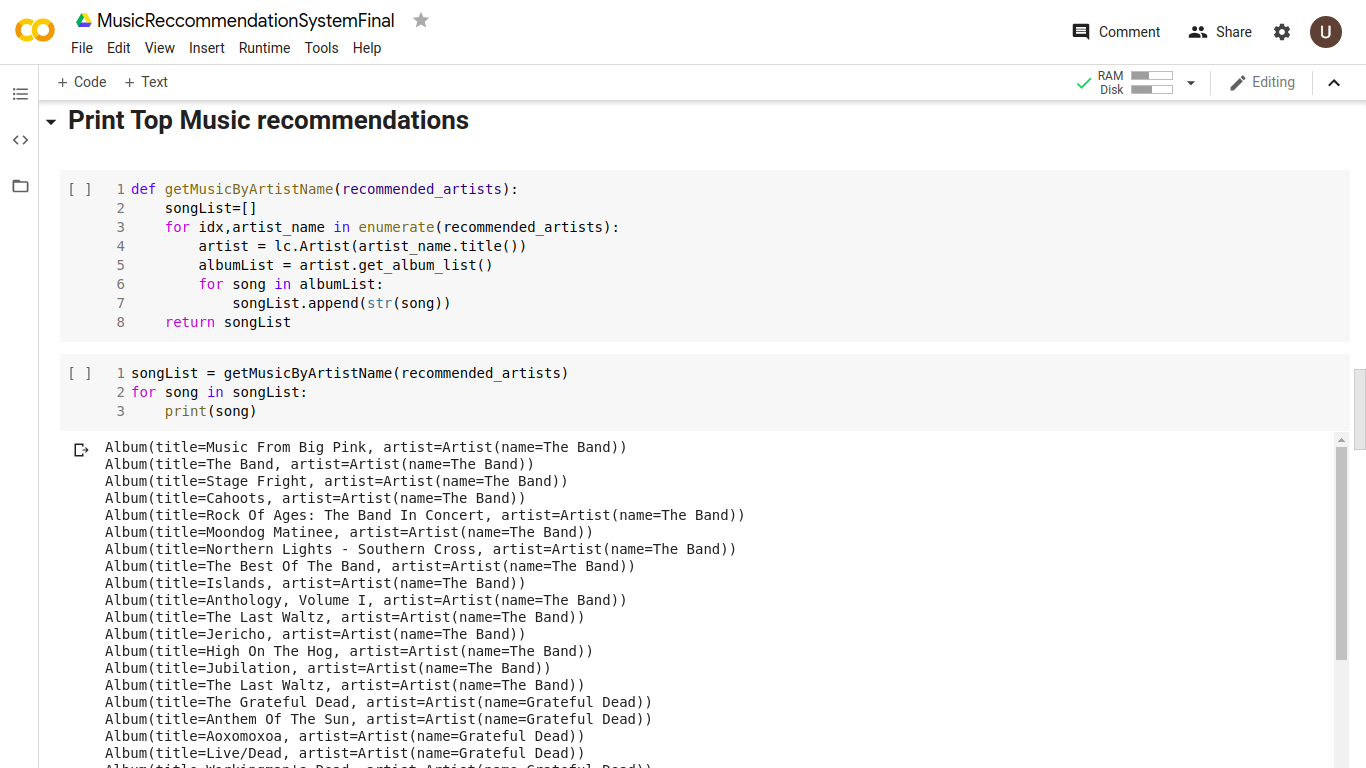
\includegraphics[scale=.8]{report/recommendedMusic.png}
\caption{Generated Playlist}
\label{chap0Fig:2}
\end{figure}